\documentclass[a4paper, 12pt]{article}
\usepackage[total={17cm,25cm}, top=2.5cm, left=2.5cm, right=2.5cm,  includefoot]{geometry}
\usepackage[utf8]{inputenc}
\usepackage{array}
\usepackage{multirow}
\usepackage{hhline}
\usepackage{gensymb}
\usepackage{graphicx}
\graphicspath{ {} }
\usepackage[czech]{babel}
\usepackage{enumitem}
\usepackage{pdfpages}
\usepackage{amsmath}
\usepackage{verbatim}
\usepackage{listings}
\usepackage{hyperref}
\usepackage{amssymb}


\pagestyle{empty} % vypne číslování stránek




%\usepackage[OT2,OT1]{fontenc}
\newcommand\cyr
{
\renewcommand\rmdefault{wncyr}
\renewcommand\sfdefault{wncyss}
\renewcommand\encodingdefault{OT2}
\normalfont
\selectfont
}
\DeclareTextFontCommand{\textcyr}{\cyr}
\def\cprime{\char"7E }
\def\cdprime{\char"7F }
\def\eoborotnoye{\char’013}
\def\Eoborotnoye{\char’003}


\begin{document}



\begin{titlepage}
\begin{center}
\noindent
\Large \textbf{České vysoké učení technické v Praze }\\ Fakulta stavební
\vspace{5cm}

\huge

%vložení loga cvut
%\begin{figure}[h!]
%	\centering
%	\includegraphics[width=7cm]{logo.png}
%\end{figure}

\vspace{0.5cm}

155ADKG: Digitální model terénu \\

\vspace{10cm}




\Large
Michael Kala\\
Anna Zemánková \\

\end{center}

\end{titlepage}




\pagestyle{plain}     % zapne obyčejné číslování
\setcounter{page}{1}  % nastaví čítač stránek znovu od jedné

%\tableofcontents
%\newpage

\section{Zadání}

\begin{figure}[h!]
	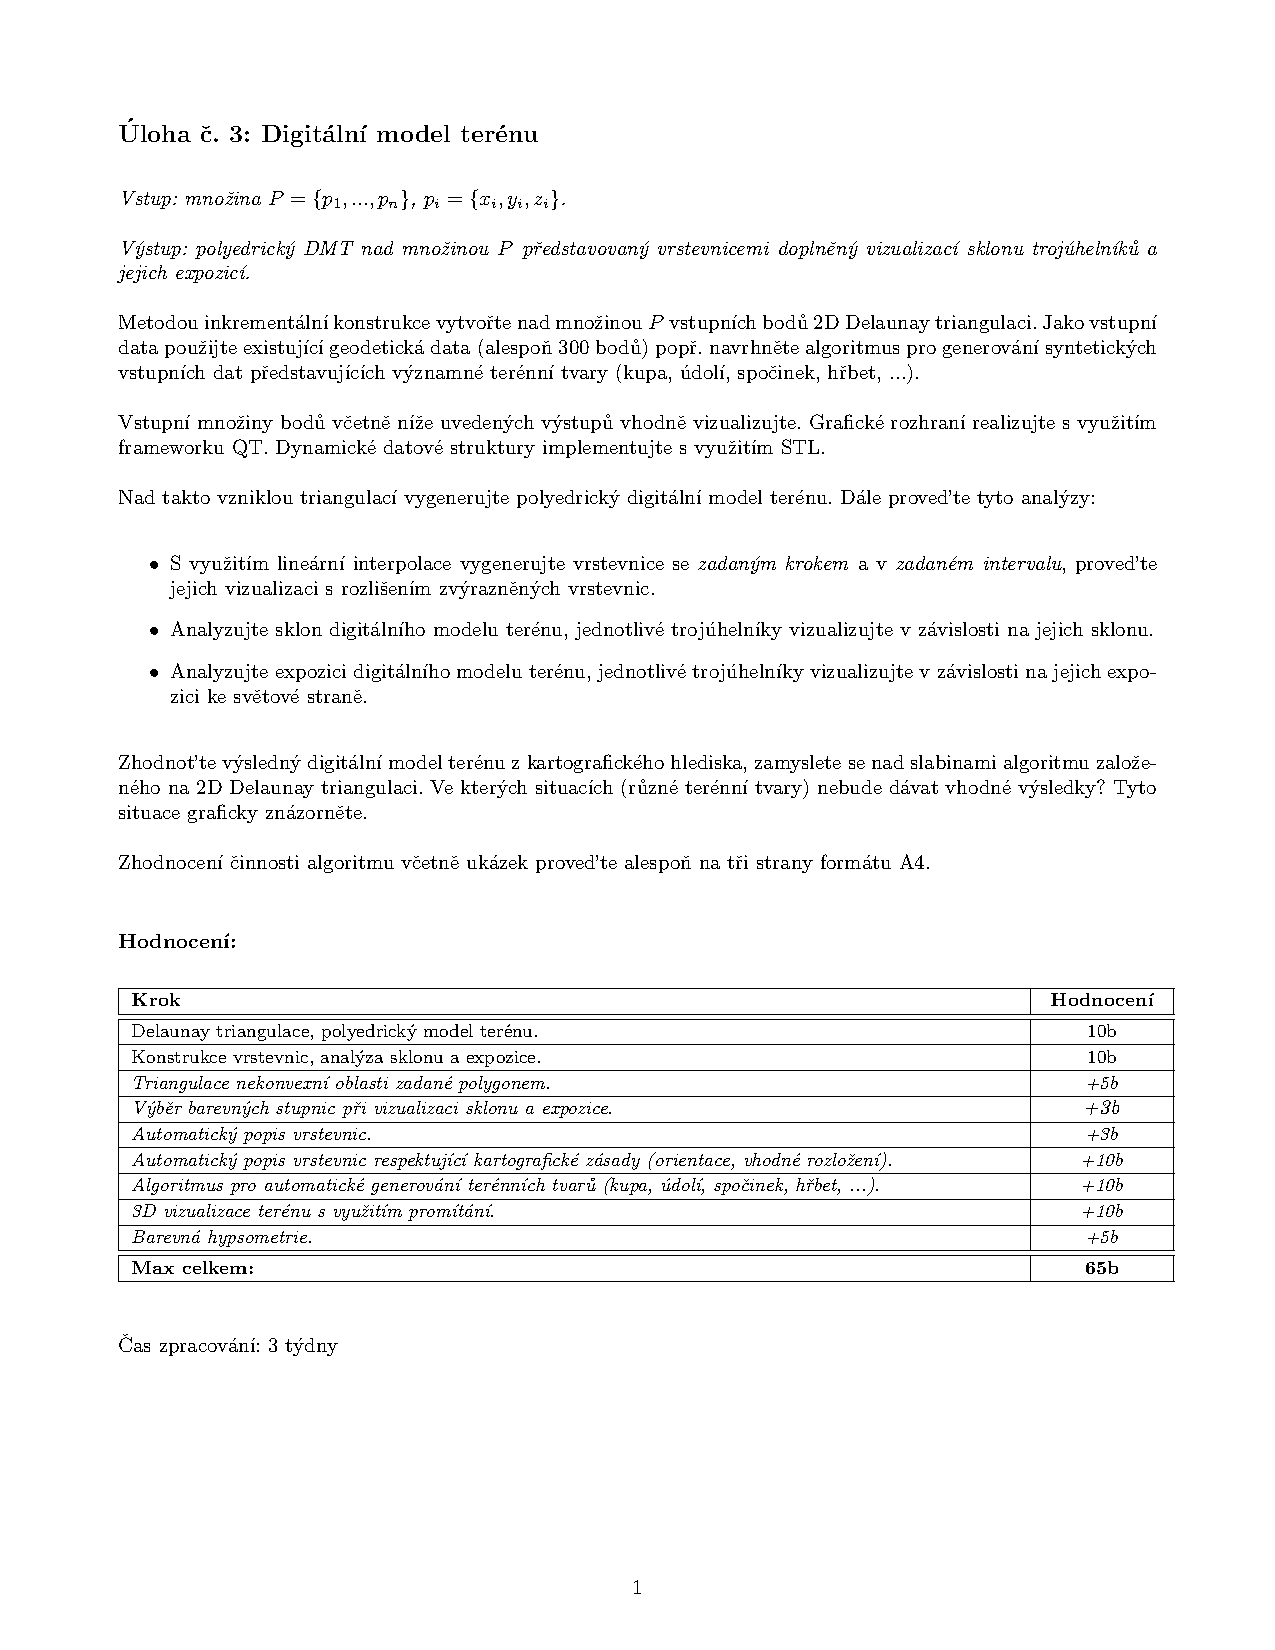
\includegraphics[clip, trim=0cm 5cm 0cm 3cm, width=1.0\textwidth]{zadani.pdf}
\end{figure}


\section{Údaje o bonusových úlohách}
Z bonusových úloh byly zpracovány:
\begin{itemize}
	\item výběr barevné stupnice při vizualizaci expozice (sklon byl vizualizován již na hodině)
	\item automatický popis vrstevnic
	\item barevná hypsometrie
\end{itemize}



\clearpage

\section{Popis a rozbor problému}

Mějme množinu bodů $P \{p_i\}$,  $p_i = \{x_i, y_i, z_i\}$. Nad touto množinou chceme vytvořit síť trojúhelníků $t_j$ pomocí Delaunay triangulace $DT$, následně vytvořit vrstevnice a pro vizualizaci DMT určit sklon a expozici jednotlivých trojúhelníků.\\ 

\subsection{Delaunay triangulace}
Vlastnosti:
\begin{itemize}
\item Uvnitř kružnice opsané trojúhelníku $t_j \in DT$ neleží žádný jiný bod množiny P.
\item $DT$ maximalizuje minimální úhel v $\forall t_j$, avšak $DT$ neminimalizuje maximální úhel v $t_j$.
\item $DT$ je lokálně optimální i globálně optimální vůči kritériu minimálního úhlu.
\item $DT$ je jednoznačná, pokud žádné čtyři body neleží na kružnici.
\end{itemize}
\vspace{1.5cm}

\subsection{Vrstevnice}
Vrstevnice byly určeny za využití lineární interpolace, při které se předpokládá, že spád terénu je mezi podrobnými body $p_i$, mezi nimiž se provádí interpolace, konstantní.\\

Mějme trojúhelník $t_j$, tvořený hranami $e_1, e_2, e_3$ a rovinu vrstevnice $\rho$ o dané výšce.

Vztah hrany tojúhelníku a roviny vrstevnice:
\begin{enumerate}
\item $(z-z_i)*(z-z_{i+1}) < 0$  $\longrightarrow e_i \cap \rho$
\item $(z-z_i)*(z-z_{i+1}) > 0$  $\longrightarrow e_i \notin \rho$ 
\item $(z-z_i)*(z-z_{i+1}) = 0$  $\longrightarrow e_i \in \rho$
\end{enumerate}

\noindent Pokud  $e_1, e_2, e_3 \in \rho$, jedná se o trojúhelník náležící rovině $\rho$ a není nutné vrstevnici pro tento trojúhelník řešit.\\
Jestliže $e_i \cap \rho$, je vypočten průsečík hrany $e_i = (p_1, p_2)$ a roviny vrstevnice $\rho$ o výšce $z$:
$$ x = \frac{(x_2-x_1)}{(z_2-z_1)}(z-z_1)+x_1, $$
$$ y = \frac{(y_2-y_1)}{(z_2-z_1)}(z-z_1)+y_1.$$
\clearpage

\subsection{Sklon}

Sklon je úhel $\varphi$ mezi svislicí $n$ a normálou trojúhelníku $n_t$. Rovina trojúhelníku $t_j$ je určena vektory u,v.\\

\noindent$$n = (0,0,1)$$
$$n_t = \vec{u}\times \vec{v}$$
$$\varphi =\arccos(\frac{n_t  n}{|n_t| |n|})$$



\subsection{Expozice}
Expozice je orientace trojúhelníku vůči světovým stranám.\\
$$A = \arctan2(\frac{n_x}{n_y});$$ kde $n_x, n_y$ jsou vektorové součiny $u$ a $v$.\\

\noindent Expozice je vizualizována pomocí barevného spektra, barvy byly vybrány stejně jako v SW ArcMAP - ESRI:\\
\begin{figure}[h]
	\centering
	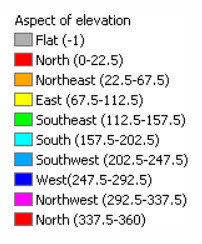
\includegraphics[width=4cm]{expozice.jpg}
	\caption{Vizualizace expozice}
\end{figure}


\clearpage
\section{Popis algoritmů}

\subsection{Delaunayova triangulace}
Triangulace byla realizována metodou inkrementální konstrukce, body jsou tedy do triangulace přidávány postupně a to tak, aby vybraný bod ležel v levé polorovině od orientované hrany, poloměr opsané kružnice byl minimální a zároveň jsou preferovány body, jejichž střed opsané kružnice leží v pravé polorovině. Pokud žádný bod těmto kritériím nevyhovuje, je orientace hrany obrácena a bod je vybírán znovu. Jakmile je bod nalezen, jsou k němu vytvořeny orientované hrany a vše je uloženo do triangulace.\\
Pro "manipulaci" s hranami se používá struktura Active Edges List $AEL$, do ní jsou ukládány hrany, ke kterým je třeba nalézt třetí bod a vytvořit trojúhelník. Jakmile je $AEL$ prázdná, algoritmus končí.

\subsubsection{Implementace metody}
\begin{enumerate}
\item $ p_1 = rand(P), ||p_2-p_1|| = min $ ....náhodný a nebližší bod
\item Vytvoř hranu $ e = (p_1,p_2) $ 
\item Inicializuj: $p_{min} = arg min_{\forall p_i\in\sigma_L(e)} r'(k_i), k_i = (a, b, p_i), e = (a,b)$
\item Pokud $ \nexists p_{min},$ prohoď orientaci $e \longleftarrow (b,a) $. Jdi na $3)$
\item $e_2 = (p_1,p_{min}), e_3 = (p_{min},p_1) $...zbývající hrany trojúhelníku
\item $AEL \longleftarrow e, AEL \longleftarrow e_2, AEL \longleftarrow e_3 $
\item $DT \longleftarrow e, DT \longleftarrow e_2, DT \longleftarrow e_3 $ 
\item while AEL not empty:
\item \hspace {1cm} $AEL  \longrightarrow e, e = (p_1, p_2) $....vezme první hranu z AEL
\item \hspace {1cm}$ e = (p_2, p_1)$ ...prohodí její orientaci
\item \hspace {1cm} $p_{min} = arg min_{\forall p_i\in\sigma_L(e)} r'(k_i), k_i = (a, b, p_i), e = (a,b) $
\item \hspace {1cm} if $ \exists p_{min}:$
\item \hspace {2cm} $e_2 = (p_1,p_{min}), e_2 = (p_{min},p_1) $...zbývající hrany trojúhelníku
\item \hspace {2cm} $DT \longleftarrow e  $  
\item \hspace {2cm} $ add(e_2,AEL,DT), add(e_3,AEL,DT)$
\end{enumerate}
\clearpage
Dílčí algoritmus Add:
\begin{enumerate}
	\item Vytvoř hranu $e' = (b,a)$
	\item if $(e' \in AEL)$
	\item \hspace {1cm} $ AEL \longrightarrow e'$...Odstraň z AEL
	\item else:
	\item \hspace {1cm} $ AEL \longleftarrow e$ ...Přidej do AEL
	\item $DT\longleftarrow (a,b)$ Přidej do DT
\end{enumerate}

\subsubsection{Problematické situace}
Pokud je vstupními daty grid, dochází k nejednoznačnosti Delaunay triangulace - na opsané kružnici leží čtyři body. V tom případě nefunguje výpočet vrstevnic ani následných analýz.

%OBRÁZEK
%\begin{figure}[h]
%	\centering
%	\includegraphics[width=10cm]{grid.jpg}
%	\caption{Delaunay triangulace - grid}
%\end{figure}

%OBRÁZEK
%\begin{figure}[h]
%	\centering
%	\includegraphics[width=10cm]{vrstevnice_grid.jpg}
%	\caption{Vrstevnice - grid}
%\end{figure}

%OBRÁZEK
%\begin{figure}[h]
%	\centering
%	\includegraphics[width=10cm]{sklon_grid.jpg}
%	\caption{Sklon - grid}
%\end{figure}
\clearpage

% ===============================================================

\section{Vstupní data}

Vstupními daty je textový soubor \textit{*.txt} se souřadnicemi bodů ve tvaru [X,Y,Z]. Lze jej do aplikace nahrát pomocí tlačítka \textit{Load points}.

Součástí příloh je textový soubor s testovacími daty \textit{testovaci\_data.txt}.

\section{Výstupní data}
Výsledky aplikace jsou vizualizovány v kanvasu grafického rozhraní.

%OBRÁZEK
%\begin{figure}[h]
%	\centering
%	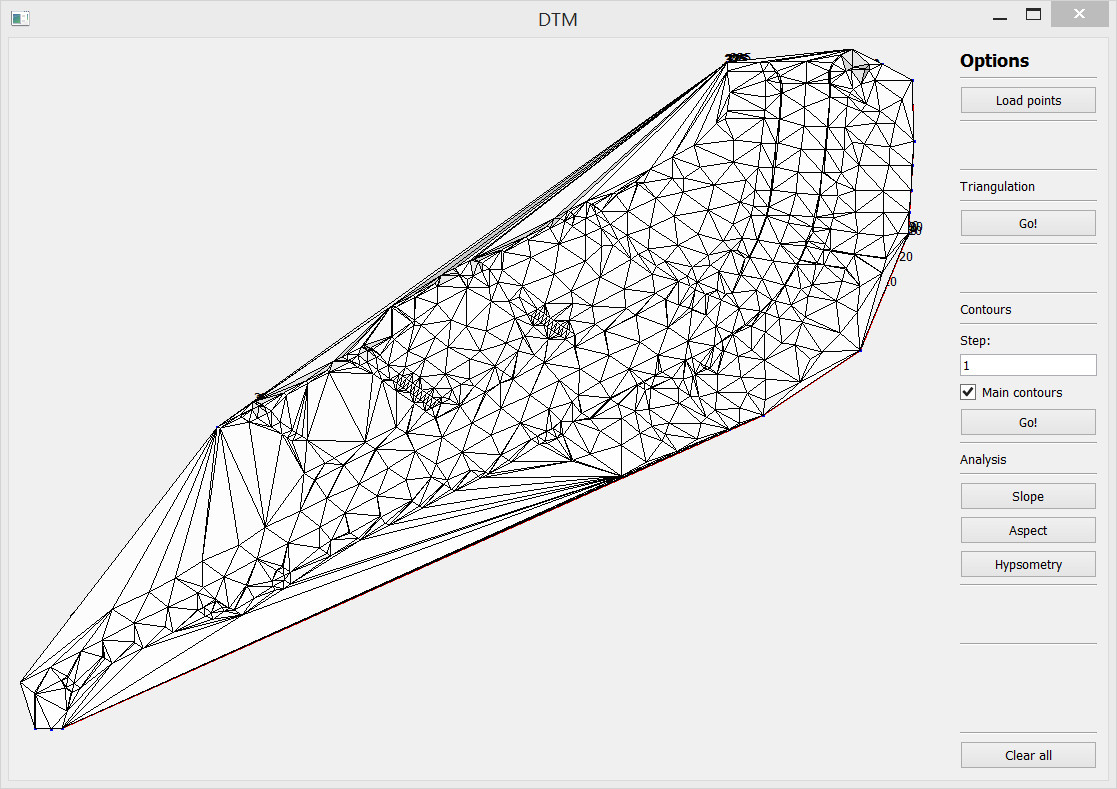
\includegraphics[width=10cm]{sklon.jpg}
%	\caption{Sklon}
%\end{figure}

\clearpage

\section{Ukázka vytvořené aplikace}


%OBRÁZEK
\begin{figure}[h]
	\centering
	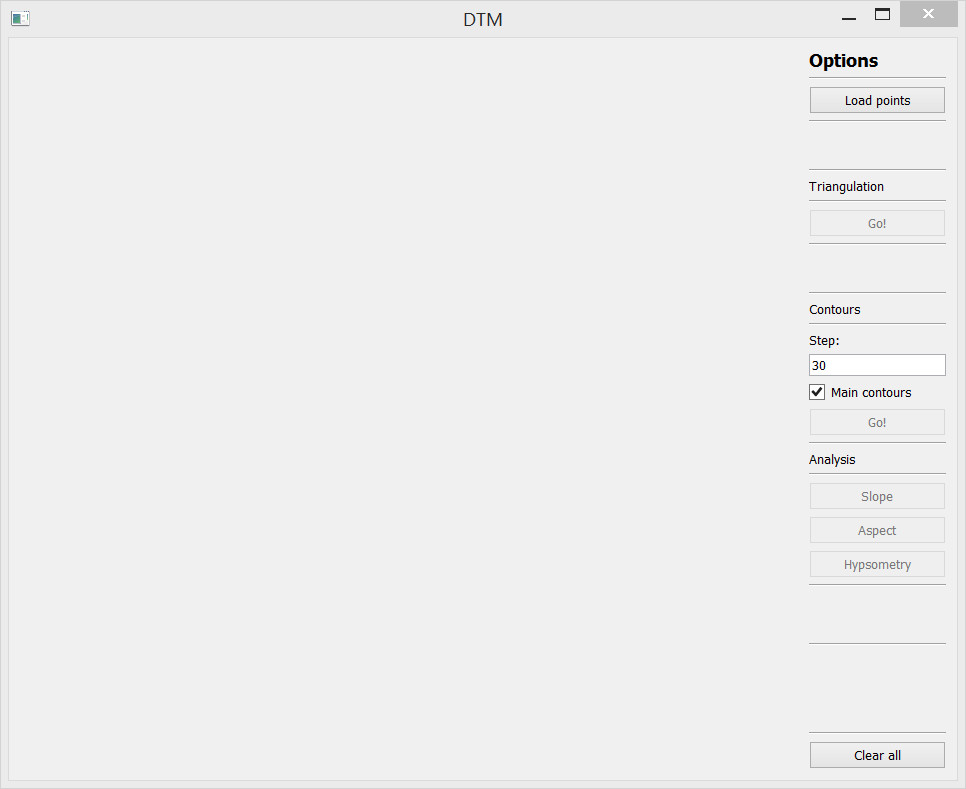
\includegraphics[width=10cm]{aplikace.jpg}
	\caption{Rozvržení aplikace}
\end{figure}

Nejprve je třeba nahrát vstupní data pomocí tlačítka \textit{Load points} a následně je možné vypočítat Delaunay triangulaci, teprve poté jsou zpřístupněna i ostatní tlačítka aplikace. \\

%OBRÁZEK
%\begin{figure}[h]
%	\centering
%	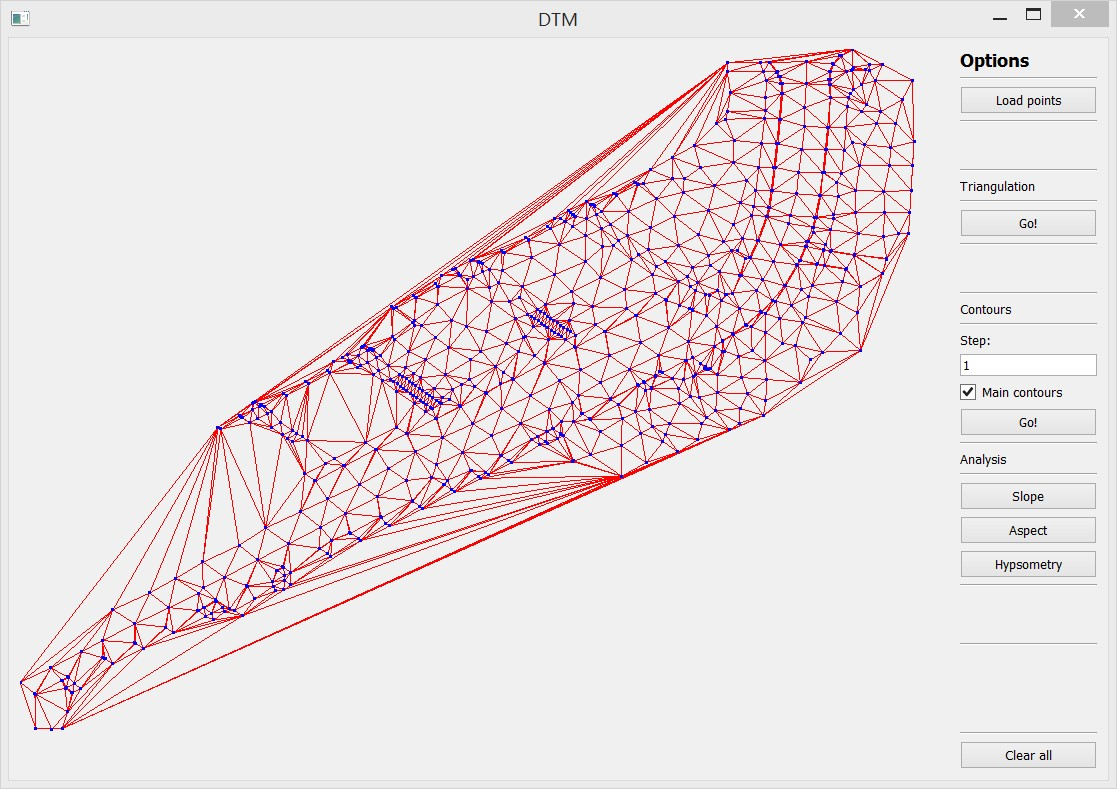
\includegraphics[width=10cm]{DT.jpg}
%	\caption{Delaunay triangulace}
%\end{figure}

Při výpočtu vrstevnic je třeba zadat krok vrstevnic a (ne)zaškrtnout zvýraznění hlavních vrstevnic.

%OBRÁZEK
%\begin{figure}[h]
%	\centering
%	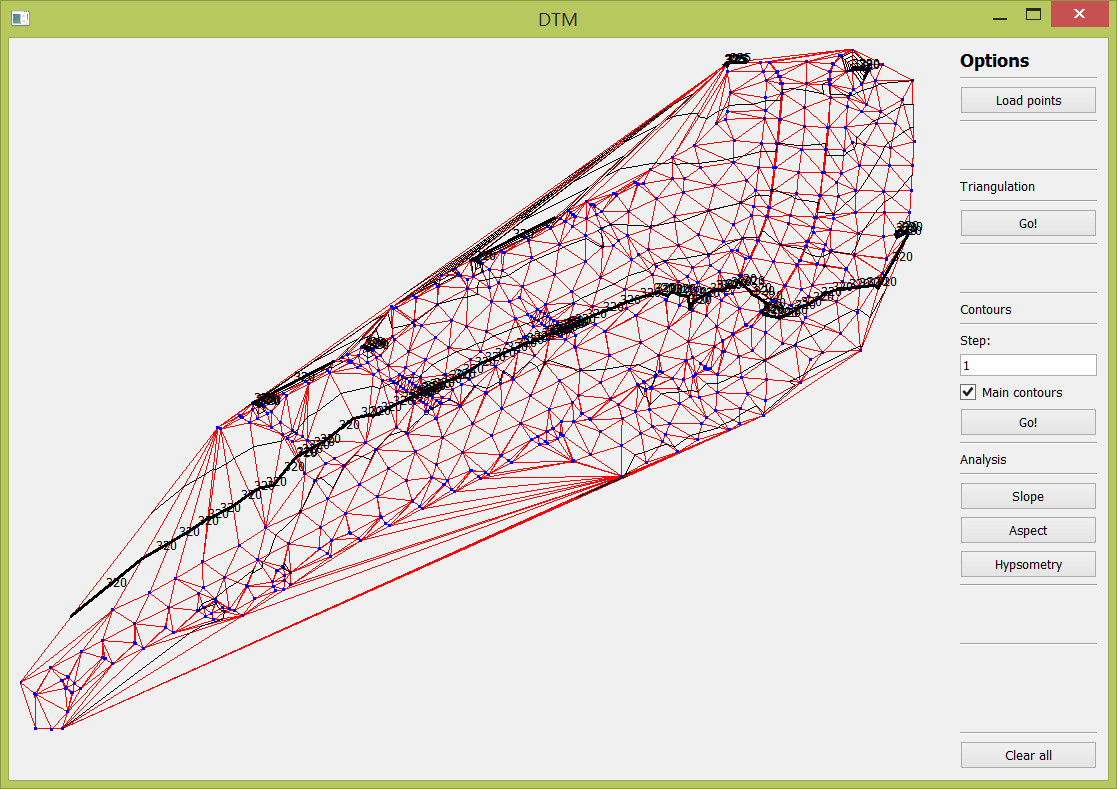
\includegraphics[width=10cm]{vrstevnice.jpg}
%	\caption{Vrstevnice}
%\end{figure}

V sekci analysis je možné vypočíst a vizualizovat sklon a expozici.
%OBRÁZEK
%\begin{figure}[h]
%	\centering
%	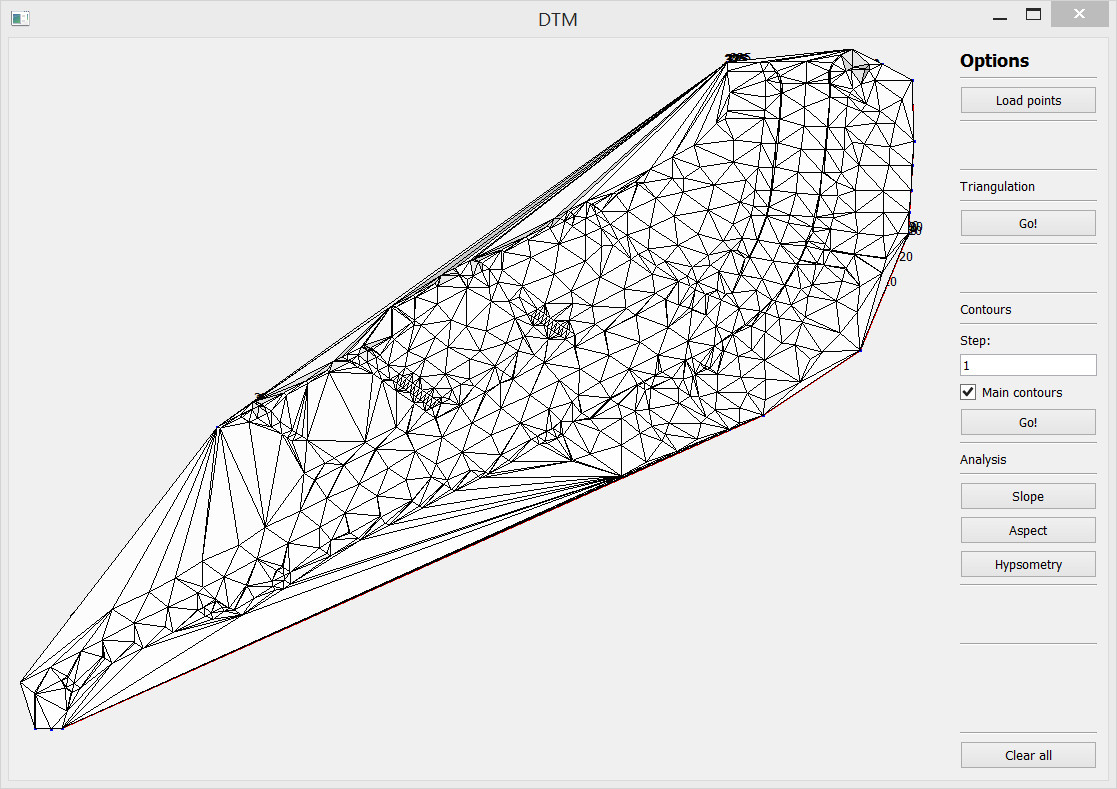
\includegraphics[width=10cm]{sklon.jpg}
%	\caption{Sklon}
%\end{figure}

%OBRÁZEK
%\begin{figure}[h]
%	\centering
%	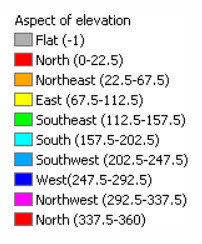
\includegraphics[width=10cm]{expozice.jpg}
%	\caption{Expozice}
%\end{figure}

Vše je uvedeno do původního stavu (smazány body i vypočtené výsledky) kliknutím na tlačítko Clear.\\
\clearpage





\clearpage

%=======================================================================================

\section {Dokumentace}

\subsection{Algorithms}
V třídě Algorithms jsou staticky implementovány algoritmy počítající Delaunay triangulaci, vrstevnice, analýzu DMT (sklon a expozici) - a barevnou hypsometrii. 

\begin{itemize}

	\item Výčtový typ \textbf{TPosition}
		\begin{itemize}
			\item Typ využitý jako návratová hodnota členské metody \textbf{getPointLinePosition}.
			\item \textbf{LEFT = 0}
			\item \textbf{RIGHT = 1}
			\item \textbf{ON = 2}
		\end{itemize}

	\item Metoda \textbf{getPointLinePosition}
		\begin{itemize}
			\item Tato metoda slouží k určení polohy bodu vůči přímce. Návratovou hodnotou je výčtový typ \textbf{TPosition}.
			\item Vstup
				\begin{itemize}
					\item \textbf{QPointF \&q} - určovaný bod
					\item \textbf{QPointF \&a, \&b} - body přímky
				\end{itemize}
			\item Výstup
				\begin{itemize}
					\item \textbf{LEFT} - bod vlevo od přímky
					\item \textbf{RIGHT} - bod vpravo od přímky
					\item \textbf{ON} - bod na přímce
				\end{itemize}

		\end{itemize}


	\item Metoda \textbf{getCircleRadius}
		\begin{itemize}
			\item Tato metoda slouží k výpočtu poloměru opsané kružnice \textbf{double}.
			\item Vstup
				\begin{itemize}
					\item \textbf{QPoint3D \&p1, \&p2, \&p3, \&c} - body $p_i$ jsou body, jimž je kružnice opsána, do bodu c jsou ukládány souřadnice středu kružnice.
				\end{itemize}
			\item Výstup
				\begin{itemize}	
					\item Vypočtený poloměr kružnice.
				\end{itemize}
		\end{itemize}	
		
	\item Metoda \textbf{getNearestPoint}		
	\begin{itemize}
		\item Tato metoda slouží k vyhedání nejbližšího bodu. \textbf{int}.
		\item Vstup
		\begin{itemize}
			\item \textbf{QPoint3D \&p, std::vector$<$QPoint3D$>$ \&points} - od bodu $p$ je hledán nejbližší bod z vektoru bodů $points$.
		\end{itemize}
		\item Výstup
		\begin{itemize}	
			\item index nejbližšího bodu.
		\end{itemize}
	\end{itemize}	
	
	\item Metoda \textbf{distance}		
	\begin{itemize}
		\item Tato metoda slouží k výpočtu vzdálenosti dvou bodů. \textbf{double}.
		\item Vstup
		\begin{itemize}
			\item \textbf{QPoint3D \&p1, QPoint3D \&p2} 
		\end{itemize}
		\item Výstup
		\begin{itemize}	
			\item vzdálenost dvou bodů.
		\end{itemize}
	\end{itemize}

	\item Metoda \textbf{getDelaunayPoint}		
\begin{itemize}
	\item Tato metoda slouží k vyhledání bodu, který vyhovuje kritériím Delaunay traingulace. \textbf{int}.
	\item Vstup
	\begin{itemize}
		\item \textbf{QPoint3D \&s, QPoint3D \&e, std::vector$<$QPoint3D$>$ \&points} 
	\end{itemize}
	\item Výstup
	\begin{itemize}	
		\item index bodu.
	\end{itemize}
\end{itemize}

	\item Metoda \textbf{DT}		
\begin{itemize}
	\item Tato metoda slouží k vytvoření vektoru, v němž jsou hrany Delaunay triangulace. \textbf{std::vector$<$Edge$>$ }.
	\item Vstup
	\begin{itemize}
		\item \textbf{std::vector$<$QPoint3D$>$ \&points} 
	\end{itemize}
	\item Výstup
	\begin{itemize}	
		\item vektor hran Delaunay triangulace.
	\end{itemize}
\end{itemize}

	\item Metoda \textbf{getContourPoint}		
\begin{itemize}
	\item Tato metoda slouží k vypočtení souřadnic průsečíku vrstevnice a hrany DT. \textbf{QPoint3D}.
	\item Vstup
	\begin{itemize}
		\item \textbf{QPoint3D \&p1,\&p2, double z} z je výška vrstevnice, bod $p_1 resp. p_2$ je počáteční resp. koncový bod hrany.
	\end{itemize}
	\item Výstup
	\begin{itemize}	
		\item průsečík vrstevnice a trojúhelníku DT.
	\end{itemize}
\end{itemize}

	\item Metoda \textbf{createContours}		
\begin{itemize}
	\item Tato metoda slouží k vypočtení vrstevnic. \textbf{std::vector$<$Edge$<$}.
	\item Vstup
	\begin{itemize}
		\item \textbf{std::vector$<$Edge$<$ \&dt,
			double z\_min, double z\_max,
			double dz,std::vector$<$double$<$ \&contour\_heights, std::vector$<$QPolygonFZ$<$\&hyps} 
	\end{itemize}
	\item Výstup
	\begin{itemize}	
		\item vektor hran vrstevnic.
	\end{itemize}
\end{itemize}

	\item Metoda \textbf{getSlope}		
\begin{itemize}
	\item Tato metoda slouží k výpočtu sklonu trojúhelníku {double}.
	\item Vstup
	\begin{itemize}
		\item \textbf{QPoint3D \&p1, \&p2, \&p3} - vrcholy trojúhelníku.
	\end{itemize}
	\item Výstup
	\begin{itemize}	
		\item sklon trojúhelníku $[^\circ]$.
	\end{itemize}
\end{itemize}

	\item Metoda \textbf{getAspect}		
\begin{itemize}
	\item Tato metoda slouží k výpočtu expozice trojúhelníku {double}.
	\item Vstup
	\begin{itemize}
		\item \textbf{QPoint3D \&p1, \&p2, \&p3} - vrcholy trojúhelníku.
	\end{itemize}
	\item Výstup
	\begin{itemize}	
		\item expozice trojúhelníku $[^\circ]$.
	\end{itemize}
\end{itemize}

	\item Metoda \textbf{analyzeDMT}		
\begin{itemize}
	\item Tato metoda slouží k vytvoření trojúhelníků a vúpočtů jejich sklonu a expozice {std::vector$<$Triangle$>$}.
	\item Vstup
	\begin{itemize}
		\item \textbf{std::vector$<$Edge$>$ \&dt} - vektor hran Delaunay triangulace.
	\end{itemize}
	\item Výstup
	\begin{itemize}	
		\item vektor trojúhelníků a jejich sklon a expozice.
	\end{itemize}
\end{itemize}

	\item Metoda \textbf{sweepLineCH}
\begin{itemize}
	\item Tato metoda slouží k výpočtu konvexní obálky pomocí algoritmu Sweep Line. Jejím výstupním typem je \textbf{QPolygonF}.
	\item Vstup
	\begin{itemize}
		\item \textbf{std::vector} $<$\textbf{QPointF}$>$ \textbf{points} - vektor bodů, kolem nichž má být vytvořená konvexní obálka.
	\end{itemize}
	\item Výstup
	\begin{itemize}
		\item Polygon obsahující kovexní obálku.
	\end{itemize} 
\end{itemize}

\end{itemize}	


\subsection{Draw}
Třída draw slouží k vykreslení načtených bodů, vypočtené Delaunay triangulace, vrstevnic, sklonu, expozice a hypsometrie. Třída dědí od třídy \textbf{QWidget}. 

\begin{itemize}
	\item Členské proměnné
		\begin{itemize}
			\item \textbf{std::vector $<$QPoint3D$>$ points } vektor načtených bodů
			\item \textbf{std::vector $<$Edge$>$ dt }- vektor hran Delaunay triangulace
			\item \textbf{std::vector $<$Edge$>$ contours} - vektor hran vrstevnic
			\item \textbf{std::vector $<$double$>$ contours\_heights} - vektor výšek vrstevnic
			\item \textbf{std::vector $<$Triangle$>$ dtm} - vektor trojúhelníků Delaunay triangulace
			\item \textbf{std::vector $<$QPolygonFZ$>$ hyps} - vektor polygonů hypsometrie
			\item \textbf{bool draw\_main} - nese informaci, zda chce uživatel vykreslit zvýraznění hlavních vrstevnic
			\item \textbf{int step} - rozestup vrstevnic
			\item \textbf{bool draw\_slope} - nese informaci, má být vykreslen sklon
			\item \textbf{bool draw\_aspect} - nese informaci, má být vykreslena expozice
			\item \textbf{bool draw\_hyps} - nese informaci, má být vykreslena hypsometrie
			\item \textbf{std::vector $<$QColor$>$ ctable} - tabulka barev pro hypsometrii
		\end{itemize}
	



	\item public metody
	\begin{itemize}
	\item Metoda \textbf{paintEvent}
		\begin{itemize}
			\item Tato metoda slouží k vykreslení načtených bodů, vypočtené Delaunay triangulace, vrstevnic, sklonu, expozice a hypsometrie. Metoda se volá pomocí metody \textbf{repaint()}. Návratovým typem je \textbf{void}.
			\item Vstup
				\begin{itemize}
					\item \textbf{QPaintEvent *e}
				\end{itemize}
		\end{itemize}

%	\item Metoda \textbf{mousePressEvent}
%		\begin{itemize}
%			\item Metoda sloužící k uložení bodu do členské proměnné \textbf{points} určeného kliknutím myší nad kreslícím plátnem. Jejím návratovým typem je \textbf{void}.	
%			\item Vstup
%				\begin{itemize}
%					\item \textbf{QMouseEvent *e}
%				\end{itemize}
%		\end{itemize}

	\item Metoda \textbf{clearDT}
		\begin{itemize}
			\item Tato metoda slouží pro vymazání bodů, triangulace, vrstevnic a hypsometrie. Na vstupu není nic a je typu void.
		\end{itemize}	

	\item Metoda \textbf{getPoints}
Tato metoda slouží k zpřístupnění členské proměnné points.


	\item Metoda \textbf{getDT}
Tato metoda slouží k zpřístupnění členské proměnné dt.
%=======================================================================================================
	\item Metoda \textbf{setDT}
Tato metoda slouží k přiřazení hodnot členské proměnné dt.

	\item Metoda \textbf{setContours}
Metoda slouží k přiřazení hodnot členským proměnným contours, sontours\_heights, step, draw\_main a hyps.

\item Metoda \textbf{setDTM}
Tato metoda slouží k přiřazení hodnot členské proměnné dtm.

	\item Metoda \textbf{loadPoints}
\begin{itemize}
	\item Tato metoda slouží pro načtení bodů z textového souboru do vetoru points a pro určení minimální a maximální výšky bodů v souboru. Zároveň je zvoleno "měřítko" kanvasu dle velikosti kanvasu a rozsahu vstupních dat. \textbf{void}.
	\item Vstup
	\begin{itemize}
		\item \textbf{std::string path, QSizeF \&canvas\_size, double \&min\_z, \&max\_z}
	\end{itemize}
\end{itemize}
%=======================================================
%Tady nevím, jak to napsat, doplniš to prosím?
%======================================================
%	\item Metoda \textbf{setDrawSlope}
%
%
%	\item Metoda \textbf{setDrawAspect}

%	\item Metoda \textbf{drawHypsometry}
%========================================================
	
	\item Metoda \textbf{genAspColor}
	Metoda slouží k přiřazení hodnot do členské proměnné ctable - zde jsou přiřazeny barvy k hodnotám expozice.


\end{itemize}
\end{itemize}


\subsection{Edge}
%=======================================================
% Doplniš to prosím?
%======================================================

\begin{itemize}
	\item členské proměnné \textbf{Qpoint3D s, e} - počáteční a koncový bod hrany
	\item public metody:
	\begin{itemize}
		\item \textbf{getS resp. getE} - metoda slouží k zpřístupnění členských proměnných s resp. e. Návratovým typem je \textbf{QPoint3D}. 
		\item \textbf{switchOr} - metoda slouží ke změně orientace hrany - prohodí počáteční a koncový bod. Návratovým typem je \textbf{void}. 
	\end{itemize}
\end{itemize}

\subsection{QPoint3D}

Implicitní hodnoty souřadnic: $[0,0,0]$
%=======================================================
% Doplniš to prosím?
%======================================================
\begin{itemize}
	\item členské proměnné \textbf{double z} - výška bodu
	\item public metody:
	\begin{itemize}
		\item \textbf{getZ} - metoda slouží k zpřístupnění členské proměnné z. Návratovým typem je \textbf{double}. 
		\item \textbf{getZ} - metoda slouží k přiřazení hodnoty do členské proměnné z. Návratovým typem je \textbf{void}. 
	\end{itemize}
\end{itemize}
%=======================================================
% Doplniš to prosím?
%======================================================
%\subsection{QPolygonFZ}

\subsection{SortByXAsc, SortByZAsc,}
Třídy sloužící jako sortovací kritérium - podle rostoucí souřadnice x resp. souřadnice y (při stejných souřadnicích x resp. y je druhým kritériem druhá souřadnice) a podle rostoucího úhlu mezi body (při stejném úhlu je druhým kritériem vzdálenosti mezi body).

%=======================================================
% Doplniš to prosím?
%======================================================
%\subsection{SortPolByZAsc}
%
\subsection{Triangle}
%=======================================================
% Doplniš to prosím?
%======================================================
\begin{itemize}
	\item členské proměnné:\\ \textbf{QPoint3D p1,p2,p3} - tři vrcholy trojúhelníku \\
	\textbf{double slope, aspect} - sklon a expozice trojúhelníku
	\item public metody:\\
	Metodami je zpřístupněna hdonota členských proměnných.
\end{itemize}


\clearpage


\subsection{Widget}
Tato třída slouží ke komunikaci s GUI. Třída dědí od třídy QWidget. Všechny její metody slouží jako sloty k signálům z GUI, nemají žádné vstupní hodnoty a jejich návratovým typem je void. 

\begin{itemize}
	\item Metoda \textbf{on\_del\_button\_clicked} - reaguje na zmáčknutí tlačítka pro vypočtení Daleunay triangulace, volá metodu \textbf{AnalyzeDTM} z třídy \textbf{Algorithms}.

	\item Metoda \textbf{on\_clear\_button\_clicked} - reaguje na zmáčknutí tlačítka pro vymazání obsahu kreslícího plátna, volá metodu \textbf{clearDT} z třídy \textbf{Draw}.
	
	\item Metoda \textbf{on\_cont\_button\_clicked} - reaguje na zmáčknutí tlačítka pro generování vrstevnic bodů, volá metodu \textbf{createContours} z třídy \textbf{Algorithms} a \textbf{setContours} z třídy \textbf{Draw}.

	\item Metoda \textbf{on\_slope\_button\_clicked} - reaguje na zmáčknutí tlačítka pro vypočet sklonu, volá metodu \textbf{setDrawSlope} z třídy \textbf{Draw}.

	\item Metoda \textbf{on\_load\_points\_button\_clicked} - reaguje na zmáčknutí tlačítka pro načtení bodů, volá metodu \textbf{loadPoints} z třídy \textbf{Draw}.
	
	\item Metoda \textbf{on\_aspect\_button\_clicked} - reaguje na zmáčknutí tlačítka pro výpočet expozice , volá metodu \textbf{setDrawAspect} z třídy \textbf{Draw}.
	
	\item Metoda \textbf{on\_hyps\_button\_clicked} - reaguje na zmáčknutí tlačítka pro vykreslení hypsometrie, volá metodu \textbf{drawHypsometry} z třídy \textbf{Draw}.

\end{itemize} 


\clearpage

\section{Přílohy}

\begin{itemize}
	\item Príloha č.1: Testovacídata - \textit{testovaci\_data.txt}.
\end{itemize}
 %--------------------------------------------------------------------------------------------------------------------------------------------------------------------------
\clearpage
\section{Závěr}

\subsection{Zhodnocení}

\subsection{Návrhy na vylepšení}


\clearpage
\section{Zdroje}

\begin{enumerate}
\item  BAYER, Tomáš. 2D triangulace, DMT [online][cit. 1.12.2018]. \\
Dostupné z: https://web.natur.cuni.cz/~bayertom/images/courses/Adk/adk5.pdf  \\

\item  BAYER, Tomáš. 2D triangulace, DMT [online][cit. 30.11.2018]. \\
Dostupné z: https://web.natur.cuni.cz/~bayertom/images/courses/Adk/adkcv3.pdf\\

\item Tools: Aspect. ArcMap|ArcGIS Desktop [online]. Environmental Systems Research Institute, 2016 [cit. 2018-12-02]. \\
Dostupné z: http://desktop.arcgis.com/en/arcmap/10.3/tools/spatial-analyst-toolbox/how-aspect-works.htm\\
%=======================================================================================
\end{enumerate}

\end{document}



 
